\documentclass[a4paper,10pt]{article}
\usepackage[utf8]{inputenc}

\title{Documentation for Half-Cheetah Control/Planning Using Mixed-Integer Optimization}
\author{Jiayi Wang}
\setlength{\parindent}{2em}
%\textwidth=15cm
\usepackage{indentfirst}

\addtolength{\oddsidemargin}{-.875in} %-.875
\addtolength{\evensidemargin}{-.875in}%-.875
\addtolength{\textwidth}{1.75in}%1.75

\addtolength{\topmargin}{-.875in}
\addtolength{\textheight}{1.75in}

\usepackage{graphicx}
\graphicspath{ {figures/} }

\PassOptionsToPackage{fleqn}{amsmath}		% math environments and more by the AMS 
\usepackage{amsmath}

\begin{document}

\maketitle

\section{Optimization Problem Formulation}

\subsection{Variables Definitions}

\begin{figure}[h!]
	\centering
	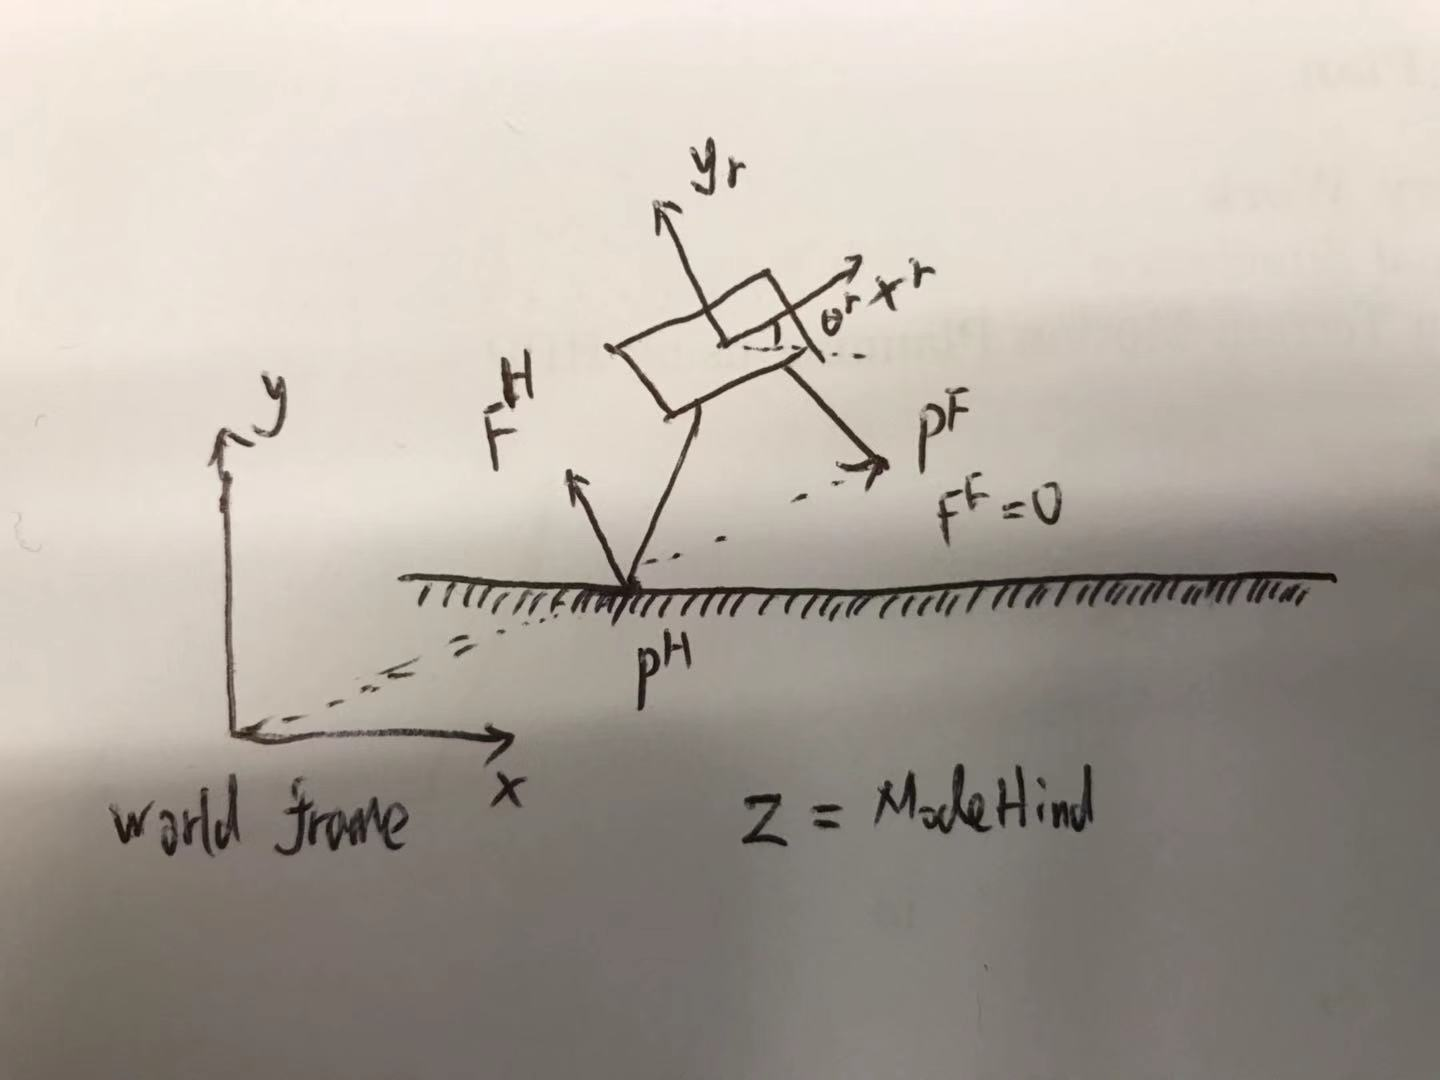
\includegraphics[scale = 0.3]{variable_definitions}
	\caption{Variable Definition for the Half Cheetah Robot}
	\label{fig:variable_definitions}
\end{figure}

Variables:
\vspace{2mm}

Robot State: $r = [x_r,y_r,\dot{x_r},\dot{y_r}]$
\vspace{2mm}

Foot/End-effector States \textbf{(IN WORLD FRAME)}: 

FrontLeg: $P^F=[P^F_x,P^F_y,\dot{P}^F_x,\dot{P}^F_y]$

HindLeg: $P^H=[P^H_x,P^H_y,\dot{P}^H_x,\dot{P}^H_y]$
\vspace{2mm}

where $P^i_x$ and $P^i_y$ are the positions of $i^{th}$ foot/end-effector, $i \in F, H$.
$\dot{P}^i_x$ and $\dot{P}^i_y$ are the velocities of $i^{th}$ foot/end-effector, $i \in F, H$.

\vspace{3mm}

Foot-Ground Reaction Forces \textbf{(IN WORLD FRAME)}:

FrontLeg: $F^F=[F^F_x,F^F_y]$

HindLeg: $F^H=[F^H_x,F^H_y]$
\vspace{2mm}

Mode Selection (Two Tracks):

\begin{itemize}
	\item Mode Enumeration: $Mode = [Mode^{fly},Mode^{double},Mode^{front},Mode^{hind}]$, where $Mode^i = 0,1$
	
	\item (Preferred) Define Contact Configuration for Every Foot: $C = [C^F, C^H]$, where $C^i = 0,1$
	
	Because we can just keep dynamic constraints invariant, and constrain different foot-ground reaction forces based on foot-ground contact indicators. However, the Mode Enumeration is tedious because we need to write different dynamics, footstep locations, foot-ground reaction forces constraints (big-M) based on mode indicator variables
	
\end{itemize}

\subsection{Objective/Cost Function and Constraints}

\subsubsection{Objective/Cost Function}

Quadratic form: $c = v^TQv$

where $v$ is the decision variable vector, it should be a column vector, $Q$ is the selection matrix for the Quadratic Form.

\vspace{2mm}
$v^TQv = v_1Q_{11}v_1 + v_1Q_{12}v_2 + ... + v_2Q_{21}v_1 + v_2Q_{22}v_2 + ...$

$Q_{i,j} \in R^{dim(v_i) x dim(v_j)}$ %make better

\subsubsection{Constraints}

System Dynamics:

$m\ddot{x} = F^F_x + F^H_x \rightarrow \ddot{x} = \frac{F^F_x}{m} + \frac{F^H_x}{m} \rightarrow \ddot{x} = f_x()$
\vspace{2mm}

$m\ddot{y} = -my + F^F_y + F^H_y \rightarrow \ddot{y} = -g + \frac{F^F_y}{m} + \frac{F^H_y}{m} \rightarrow \ddot{y} = f_y()$

\vspace{2mm}

Trapezoidal Collocation:

$x_{k+1}-x_k = \frac{1}{2}h_k(f_{k+1}+f_k) \rightarrow x_{k+1}-x_k-\frac{1}{2}h_kf_{k+1}-\frac{1}{2}h_kf_k = 0$

\vspace{2mm}

Apply Trapezoidal Collocation into translational dynamics:

x-axis position: $x_{k+1}-x_k=\frac{1}{2}h_k(\dot{x}_{k+1}+\dot{x}_k) \rightarrow x_{k+1}-x_k-\frac{1}{2}h_k\dot{x}_{k+1}-\frac{1}{2}h_k\dot{x}_k = 0$

x-axis velocity: 

$\dot{x}_{k+1}-\dot{x}_k-\frac{1}{2}h_k(\frac{F^F_{x,k+1}}{m}+\frac{F^H_{x,k+1}}{m})-\frac{1}{2}h_k(\frac{F^F_{x,k}}{m}+\frac{F^H_{x,k}}{m}) = 0 \rightarrow$

$\dot{x}_{k+1}-\dot{x}_k-\frac{1}{2}h_k\frac{F^F_{x,k+1}}{m}-\frac{1}{2}h_k\frac{F^H_{x,k+1}}{m}-\frac{1}{2}h_k\frac{F^F_{x,k}}{m}-\frac{1}{2}h_k\frac{F^H_{x,k}}{m} = 0$

With on/off signals (Contact or not flag):
$\dot{x}_{k+1}-\dot{x}_k-\frac{1}{2}h_k\frac{F^F_{x,k+1}}{m}C^F_{k+1}-\frac{1}{2}h_k\frac{F^H_{x,k+1}}{m}C^H_{k+1}-\frac{1}{2}h_k\frac{F^F_{x,k}}{m}C^F_{k}-\frac{1}{2}h_k\frac{F^H_{x,k}}{m}C^H_{k} = 0$

They are linear constraints

\vspace{3mm}

y-axis position: $y_{k+1}-y_k = \frac{1}{2}h_k(\dot{y}_{k+1}+\dot{y}_k) \rightarrow y_{k+1}-y_k-\frac{1}{2}h_k\dot{y}_{k+1}-\frac{1}{2}h_k\dot{y}_k = 0$

y-axis velocity:

$\dot{y}_{k+1}-\dot{y}_k-\frac{1}{2}h_k(-g+\frac{F^F_{y,k+1}}{m}+\frac{F^H_{y,k+1}}{m})-\frac{1}{2}h_k(-g+\frac{F^F_{y,k}}{m}+\frac{F^H_{y,k}}{m}) = 0 \rightarrow $

$\dot{y}_{k+1}-\dot{y}_k + \frac{1}{2}h_kg - \frac{1}{2}h_k\frac{F^F_{y,k+1}}{m} - \frac{1}{2}h_k\frac{F^H_{y,k+1}}{m} + \frac{1}{2}h_kg - \frac{1}{2}h_k\frac{F^F_{y,k}}{m} - \frac{1}{2}h_k\frac{F^H_{y,k}}{m} = 0 \rightarrow$

$\dot{y}_{k+1}-\dot{y}_k  - \frac{1}{2}h_k\frac{F^F_{y,k+1}}{m} - \frac{1}{2}h_k\frac{F^H_{y,k+1}}{m}  - \frac{1}{2}h_k\frac{F^F_{y,k}}{m} - \frac{1}{2}h_k\frac{F^H_{y,k}}{m} = - h_kg$

With on/off signals (Contact or not flag):
$\dot{y}_{k+1}-\dot{y}_k  - \frac{1}{2}h_k\frac{F^F_{y,k+1}}{m}C^F_{k+1} - \frac{1}{2}h_k\frac{F^H_{y,k+1}}{m}C^H_{k+1}  - \frac{1}{2}h_k\frac{F^F_{y,k}}{m}C^F_{k} - \frac{1}{2}h_k\frac{F^H_{y,k}}{m}C^H_{k} = - h_kg$

\vspace{3mm}

Foot/End-effector Dynamics:

Front Leg:

FrontLeg x-axis: 

$P^F_{x,k+1}-P^F_{x,k} = \frac{1}{2}h_k(\dot{P}^F_{x,k+1}+\dot{P}^F_{x,k}) \rightarrow P^F_{x,k+1}-P^F_{x,k} - \frac{1}{2}h_k\dot{P}^F_{x,k+1} - \frac{1}{2}h_k\dot{P}^F_{x,k}  = 0$

\vspace{2mm}

FrontLeg y-axis:

$P^F_{y,k+1}-P^F_{y,k} = \frac{1}{2}h_k(\dot{P}^F_{y,k+1}+\dot{P}^F_{y,k}) \rightarrow P^F_{y,k+1}-P^F_{y,k} - \frac{1}{2}h_k\dot{P}^F_{y,k+1} - \frac{1}{2}h_k\dot{P}^F_{y,k}  = 0$

\vspace{3mm}

Hind Leg:

HindLeg x-axis:

$P^H_{x,k+1}-P^H_{x,k} = \frac{1}{2}h_k(\dot{P}^H_{x,k+1}+\dot{P}^H_{x,k}) \rightarrow P^H_{x,k+1}-P^H_{x,k} - \frac{1}{2}h_k\dot{P}^H_{x,k+1} - \frac{1}{2}h_k\dot{P}^H_{x,k}  = 0$

\vspace{2mm}

HindLeg y-axis:

$P^H_{y,k+1}-P^H_{y,k} = \frac{1}{2}h_k(\dot{P}^H_{y,k+1}+\dot{P}^H_{y,k}) \rightarrow P^H_{y,k+1}-P^H_{y,k} - \frac{1}{2}h_k\dot{P}^H_{y,k+1} - \frac{1}{2}h_k\dot{P}^H_{y,k}  = 0$

\vspace{3mm}

Complementarity Constraint:
\vspace{2mm}

General Idea:

\begin{itemize}
	\item if $C = 1 \rightarrow $ foot in contact, then
		
		\begin{itemize}
			\item Foot stay on the ground: $P_y = 0$ or $P_y = height(P_x,Py)$ (terrain height map)
			\item Vertical force pointing upwards: $F_y \geq 0$
			\item Non-slippage: $\dot{P}_x = 0, \dot{P}_y =0$ (may remove if we want slippage dynamics in the future) (SEE if there are other better way to define end-effector velocity)
			
			May use logical variables, $z_{k+1}$ and $z_{k} = 0/1?$ to identify phase boundaries and knots inside a phase.
		\end{itemize}
	
	\item if $C =0 \rightarrow $ foot in the air, then
	
		\begin{itemize}
			\item No forces: $F_x = 0, F_y =0$
			\item Foot above the terrain: $P_y \geq 0$
		\end{itemize}
\end{itemize}

In Optimizer Constraint Form:

\begin{itemize}
	\item Foot/End-effector position:
	
	$P_y \leq height + M(1-C)$
	
	$P_y \geq height$
	
	\item Foot/End-Effector Velocity:
	
	x-axis:
	
	$\dot{P}_x \leq 0 + M(1-C)$
	
	$\dot{P}_x \geq 0 - M(1-C)$
	
	y-axis:
	
	$\dot{P}_y \leq 0 + M(1-C)$
	
	$\dot{P}_y \geq 0 - M(1-C)$
	
	\item Foot-ground reaction forces:
	
	x-axis:
	
	$F_x \leq 0 + MC$
	
	$F_x \geq 0 - MC$
	
	y-axis:
	
	$F_y \leq 0 + MC$
	
	$F_y \geq 0$
	
\end{itemize}

\vspace{3mm}

Complete form for Programming:

Front Leg:

\begin{itemize}
	\item Foot/End-Effector Position:
	
	$P^F_y \leq height + M^{pos}_y(1-C^F) \rightarrow P^F_y +  M^{pos}_yC^F \leq height + M^{pos}_y$
	
	$P^F_y \geq height$
	
	\item Foot/End-effector Velocity:
	
	x-axis:
	
	$\dot{P}^F_x \leq 0 + M_{vel}(1-C^F) \rightarrow \dot{P}^F_x + M_{vel}C^F \leq 0 + M_{vel}$
	
	$\dot{P}^F_x \geq 0 - M_{vel}(1-C^F) \rightarrow \dot{P}^F_x - M_{vel}C^F \geq 0 - M_{vel}$
	
	y-axis:
	
	$\dot{P}^F_y \leq 0 + M_{vel}(1-C^F) \rightarrow \dot{P}^F_y + M_{vel}C^F \leq 0 + M_{vel}$
	
	$\dot{P}^F_y \geq 0 - M_{vel}(1-C^F) \rightarrow \dot{P}^F_y - M_{vel}C^F \geq 0 - M_{vel}$
	
	\item Foot-Ground Reaction Forces:
	
	x-axis:
	
	$F^F_x \leq 0 + M_{fx}C^F \rightarrow F^F_x - M_{fx}C^F \leq 0$
	
	$F^F_x \geq 0 - M_{fx}C^F \rightarrow F^F_x + M_{fx}C^F \geq 0$
	
	y-axis:
	
	$F^F_y \leq 0 + M_{fy}C^F \rightarrow F^F_y - M_{fy}C^F \leq 0$
	
	$F^F_y \geq 0$
	
\end{itemize}

Hind Leg:

\begin{itemize}
	\item Foot/End-Effector Position:
	
	$P^H_y \leq height + M^{pos}_y(1-C^H) \rightarrow P^H_y +  M^{pos}_yC^H \leq height + M^{pos}_y$
	
	$P^H_y \geq height$
	
	\item Foot/End-effector Velocity:
	
	x-axis:
	
	$\dot{P}^H_x \leq 0 + M_{vel}(1-C^H) \rightarrow \dot{P}^H_x + M_{vel}C^H \leq 0 + M_{vel}$
	
	$\dot{P}^H_x \geq 0 - M_{vel}(1-C^H) \rightarrow \dot{P}^H_x - M_{vel}C^H \geq 0 - M_{vel}$
	
	y-axis:
	
	$\dot{P}^H_y \leq 0 + M_{vel}(1-C^H) \rightarrow \dot{P}^H_y + M_{vel}C^H \leq 0 + M_{vel}$
	
	$\dot{P}^H_y \geq 0 - M_{vel}(1-C^H) \rightarrow \dot{P}^H_y - M_{vel}C^H \geq 0 - M_{vel}$
	
	\item Foot-Ground Reaction Forces:
	
	x-axis:
	
	$F^H_x \leq 0 + M_{fx}C^H \rightarrow F^H_x - M_{fx}C^H \leq 0$
	
	$F^H_x \geq 0 - M_{fx}C^H \rightarrow F^H_x + M_{fx}C^H \geq 0$
	
	y-axis:
	
	$F^H_y \leq 0 + M_{fy}C^H \rightarrow F^H_y - M_{fy}C^H \leq 0$
	
	$F^H_y \geq 0$
	
\end{itemize}

\vspace{3mm}

Kinematics Constraint:

\vspace{3mm}

Boundary Constraints:

Initial Condition: 

$x_0 = x(0)$

$y_0 = y(0)$

$\dot{x}_0 = 0$

$\dot{y}_0 = 0$

\vspace{2mm}

Terminal Condition:

$x_T = x(T)$

$y_T = y(T)$

$\dot{x}_T = \dot{x}(T)$

$\dot{y}_T = \dot{y}(T)$

\vspace{3mm}

\section{To-Do List}
\begin{enumerate}
	\item Add testing functions, checking by verifying matrix dimensionality.
	\item Foot/End-effector velocity constraint, is there any better to define it, to remove end-effector velocity state, using logical operations.
\end{enumerate}

\section{Example Codes}

\subsection{Motion Planning Problem for Hybrid Dynamical Systems}

Given initial state $x_{init}$, goal state $x_{goal}$ and environment model $\Omega$, generate a robot motion plan:

\begin{align}
	\pi(t) = f_{plan}(x_{init},x_{goal},\Omega), t \in [0,T]
\end{align}

For a hybrid dynamical system like legged robots, in addition to continuous variables such as joint torque and/or foot-ground reaction forces, CoM trajectory, etc., the motion plan $\pi(t)$ also needs to include the mode switching sequence $M(t)$:
\begin{align}
	\\ \pi(t) = [x(t), P_{foot}(t), \lambda(t), u(t), M(t)]
\end{align}

where $x(t)$ is the robot state, $P_{foot}(t)$ is the footstep locations, $\lambda(t)$ is the foot-ground reaction forces, $u(t)$ is the control input and \textbf{$M(t)$ is the mode (dynamics) that the robot undergoes at any time $t$}:
\begin{align}
	\\ M(t) \in \{m_1,m_2,m_3,...m_N\}, \text{Time-Indexed}
\end{align}
where the number of modes $N$ is determined by the number of different contact configurations of the robot.

\vspace{3mm}

Note: the mode switching sequence can be also represented as a series (not time-indexed):
\begin{align}
\\ M(i) \in \{m_1,m_2,m_3,...m_N\}
\end{align}
In this case scenario, after determining mode switching sequence (usually a pre-defined), it will be further augmented toward complete whole-body motion plan includes time-indexed mode switching sequences along with continuous variables (i.e. contact forces, CoM trajectory, etc.)

%We can see the mode transition as a state machine (Fig \ref{fig:Mode_Transitions}) that the mode transition happens under certain conditions (Not clear about what conditions should be).

%\begin{figure}[h!]
%	\centering
%	\includegraphics[scale = 0.7]{Mode_Transitions}
%	\caption{State Machine Description for Mode Transitions}
%	\label{fig:Mode_Transitions}
%\end{figure}

%\begin{figure}[h!]
%	\centering
%	\includegraphics[scale = 0.7]{Search_Tree}
%	\caption{An Example of the Search Tree}
%	\label{fig:Search_Tree}
%\end{figure}

\cite{posa2014direct} introduces complementarity constraints to keep the trajectory optimization formulation being consistent with respect to contact changes:
\begin{align}
& \underset{\{x(t),u(t),\lambda(t)\}}{\text{minimize}} J(x(t), u(t), \lambda(t)) \nonumber \\
& \text{subject to:} \nonumber \\
& \mathbf{\phi(x(t)) \geq 0} & \textbf{Complementarity Constraint 1}\\
& \mathbf{\lambda(t) \geq 0} & \textbf{Complementarity Constraint 2}\\
& \mathbf{\phi(x(t))^T\lambda(t) = 0} & \textbf{Complementarity Constraint 3}\\
& g(x(t), u(t), \lambda(t)) \leq 0 & \text{(Other inequility constraints)} \nonumber \\
& h(x(t), u(t), \lambda(t)) = 0 & \text{(Other equality Constraints)}
\label{eq:genearl_optimization_problem}
\end{align}

\section{Plan}

(1) Reduce the search branches

(2) One step look ahead

\medskip
\newpage
\bibliographystyle{unsrt}%Used BibTeX style is unsrt
\bibliography{sample}

\end{document}
